%
% schichten.tex -- Schichtung des Meeres
%
% (c) 2018 Prof Dr Andreas Müller, Hochschule Rapperswil
%
\documentclass[tikz]{standalone}
\usepackage{times}
\usepackage{amsmath}
\usepackage{txfonts}
\usepackage[utf8]{inputenc}
\usepackage{graphics}
\usetikzlibrary{arrows,intersections}
\usetikzlibrary{math}
\begin{document}
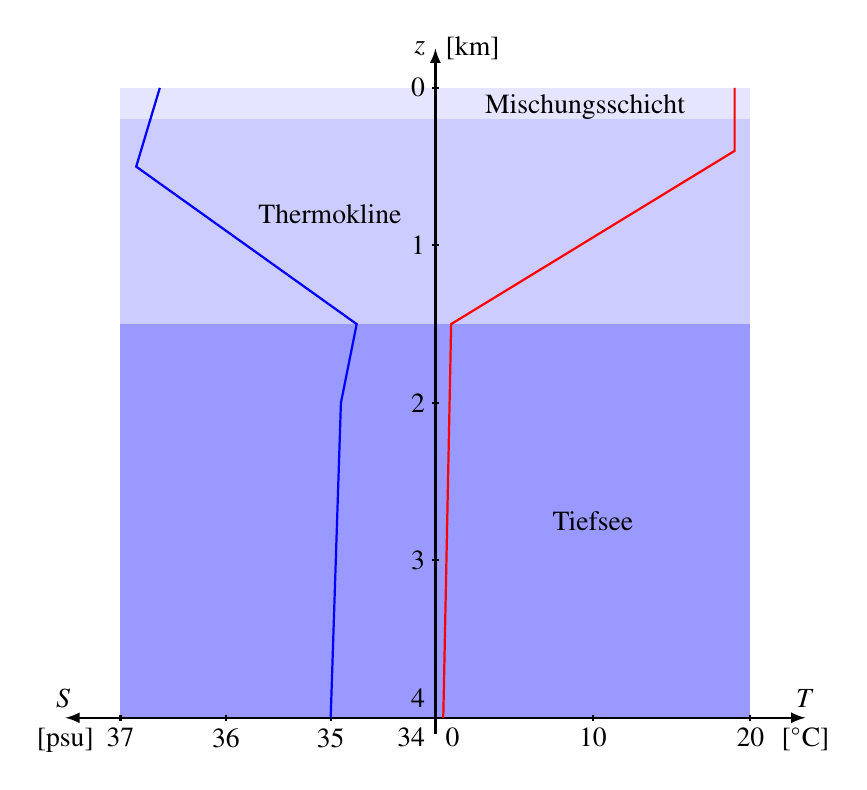
\begin{tikzpicture}[thick, >= latex]

\fill[color=blue!10] (-4,7.6)--(4,7.6)--(4,8)--(-4,8)--cycle;
\node at (0.5,7.75) [right] {Mischungsschicht};
\fill[color=blue!20] (-4,5)--(4,5)--(4,7.6)--(-4,7.6)--cycle;
\node at (-0.3,6.4) [left] {Thermokline};
\fill[color=blue!40] (-4,0)--(4,0)--(4,5)--(-4,5)--cycle;
\node at (2,2.5) {Tiefsee};

\draw[->] (0,-0.2)--(0,8.5) coordinate[label={left:$z$}];
\node at (0,8.5) [right] {$[\text{km}]$};

\draw[->] (0,0)--(4.7,0) coordinate[label=$T$];
\node at (4.7,0) [below] {$[\mathstrut^\circ\text{C}]$};
\draw[->] (0,0)--(-4.7,0) coordinate[label=$S$];
\node at (-4.7,0) [below] {$[\text{psu}]$};

\node at (0,0) [below right] {$0$};

\draw (2,-0.04)--(2,0.04);
\node at (2,0) [below] {$10$};
\draw (4,-0.04)--(4,0.04);
\node at (4,0) [below] {$20$};

\node at (0,0) [below left] {$34$};
\draw (-1.33,-0.04)--(-1.33,0.04);
\node at (-1.33,0) [below] {$35$};
\draw (-2.66,-0.04)--(-2.66,0.04);
\node at (-2.66,0) [below] {$36$};
\draw (-4,-0.04)--(-4,0.04);
\node at (-4,0) [below] {$37$};

\draw (-0.04,8)--(0.04,8);
\node at (0,8) [left] {$0$};
\draw (-0.04,6)--(0.04,6);
\node at (0,6) [left] {$1$};
\draw (-0.04,4)--(0.04,4);
\node at (0,4) [left] {$2$};
\draw (-0.04,2)--(0.04,2);
\node at (0,2) [left] {$3$};
\node at (0,0) [above left] {$4$};

\draw[color=red] (3.8,8)--(3.8,7.2)--(0.2,5)--(0.1,0);
\draw[color=blue] (-3.5,8)--(-3.8,7)--(-1,5)--(-1.2,4)--(-1.33,0);

\end{tikzpicture}
\end{document}

